% Chapter Template

\chapter{Preliminaries} % Main chapter title

\label{Chapter5} % Change X to a consecutive number; for referencing this chapter elsewhere, use \ref{ChapterX}

\lhead{Chapter 5. \emph{Preliminaries}} % Change X to a consecutive number; this is for the header on each page - perhaps a shortened title

In this chapter, we shall briefly look at all the components present in a general autonomous UAV.

\begin{figure}[h]
	\centering
	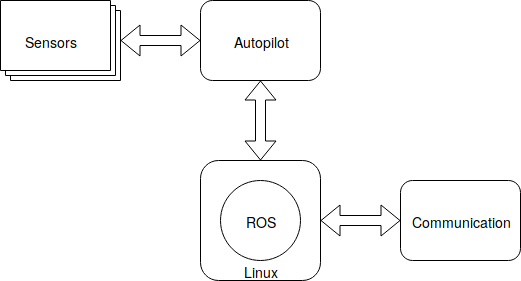
\includegraphics[scale=0.8]{Pictures/uav.png}
	\caption{Components in a general autonomous UAV}
	\label{fig: uav}
	\captionsetup{font={footnotesize,bf,it}}
\end{figure}

Figure \ref{fig: uav} shows several subsytems in an an autonomous UAV we consider. It consists of an autopilot which is handles low level control of the UAV dynamics. The autopilot is responsible for attitude stabilization, for instance, in quadrotors. It directly connects with 
 